%Version 3.1 December 2024
% See section 11 of the User Manual for version history
%
%%%%%%%%%%%%%%%%%%%%%%%%%%%%%%%%%%%%%%%%%%%%%%%%%%%%%%%%%%%%%%%%%%%%%%
%%                                                                 %%
%% Please do not use \input{...} to include other tex files.       %%
%% Submit your LaTeX manuscript as one .tex document.              %%
%%                                                                 %%
%% All additional figures and files should be attached             %%
%% separately and not embedded in the \TeX\ document itself.       %%
%%                                                                 %%
%%%%%%%%%%%%%%%%%%%%%%%%%%%%%%%%%%%%%%%%%%%%%%%%%%%%%%%%%%%%%%%%%%%%%

\documentclass[pdflatex,sn-mathphys-num]{sn-jnl}

%%%% Standard Packages
\usepackage{graphicx}%
\usepackage{multirow}%
\usepackage{amsmath,amssymb,amsfonts}%
\usepackage{amsthm}%
\usepackage{mathrsfs}%
\usepackage[title]{appendix}%
\usepackage{xcolor}%
\usepackage{textcomp}%
\usepackage{manyfoot}%
\usepackage{booktabs}%
\usepackage{algorithm}%
\usepackage{algorithmicx}%
\usepackage{algpseudocode}%
\usepackage{listings}%
\usepackage{siunitx}%
\usepackage{bm}%
\usepackage{placeins}%
\usepackage{hyperref}%
\usepackage{caption}
\usepackage{subcaption}
\usepackage{float}

%%%% Theorem styles as per the template
\theoremstyle{thmstyleone}%
\newtheorem{theorem}{Theorem}%
\newtheorem{proposition}[theorem]{Proposition}%

\theoremstyle{thmstyletwo}%
\newtheorem{example}{Example}%
\newtheorem{remark}{Remark}%

\theoremstyle{thmstylethree}%
\newtheorem{definition}{Definition}%

\raggedbottom

\begin{document}

\title[HFENet for Fine-Grained Image Classification]{HFENet: Hierarchical Feature Alignment for Data-Efficient Fine-Grained Image Classification}

\author*[1]{\fnm{XX} \sur{XX}}
\affil*[1]{\orgdiv{Department of CSE(AIML)}, \orgname{Institute of Engineering and Management}, \orgaddress{\city{Kolkata}, \postcode{700091}, \country{India}}}

\abstract{
Fine-grained image classification aims to distinguish visually similar subcategories within the same basic category, and remains challenging due to small inter-class differences and large intra-class variations. Although recent deep models have achieved promising results, their performance often degrades under limited training data because discriminative representations are difficult to learn reliably. Existing approaches have attempted to incorporate hierarchical semantic cues, such as coarse-grained labels, to facilitate fine-grained recognition. However, most of them rely on simple cascaded, parallel, or feature-fusion designs, without explicitly modeling cross-level semantic dependency or suppressing feature redundancy across branches. To address these issues, this paper proposes a hierarchical feature enhancement network (HFENet) for data-limited fine-grained image classification. The core idea is to achieve hierarchical feature alignment through cross-branch interaction between coarse-grained and fine-grained representations. Specifically, a cross-branch attention mechanism is introduced to dynamically transfer semantic guidance from the coarse branch to the fine branch, while an orthogonality regularization term is employed to reduce redundant representations and encourage complementary feature learning. In addition, a hierarchical Kullback--Leibler divergence is incorporated into the optimization objective to improve semantic consistency between branches. Experiments on CIFAR-100 show that the proposed method achieves accuracies of 70.8\%, 77.2\%, 80.5\%, and 82.7\% under 30\%, 50\%, 80\%, and 100\% training ratios, respectively. The results indicate that HFENet provides consistent improvements over the baseline dual-branch model and several representative comparison methods, especially in low-data settings. Ablation studies and visualization results further confirm the effectiveness of the proposed hierarchical alignment and redundancy suppression mechanisms.
}

\keywords{Fine-grained image classification, Hierarchical feature alignment, Cross-branch attention, Orthogonality regularization, Complementary representation learning, Data-efficient learning}

\maketitle

\section{Introduction}
\label{sec:introduction}

Fine-grained image classification (FGIC) aims to distinguish visually similar subcategories within the same basic-level category. 
Compared with generic image classification, FGIC is more challenging due to subtle inter-class differences and large intra-class variations. 
These challenges become more severe under limited training data, where models are prone to overfitting and often fail to learn robust discriminative representations.

Existing studies have attempted to improve FGIC performance by introducing attention mechanisms, multi-branch architectures, and hierarchical semantic supervision. 
Although these methods have shown promising results, two limitations still remain. 
First, the semantic relationship between coarse-grained and fine-grained representations is often not explicitly modeled. 
Most existing hierarchical methods simply concatenate or sum features from different levels without modeling the conditional dependency that coarse semantics should guide fine-grained discrimination. 
Second, multi-branch designs may introduce redundant representations, which weakens the effectiveness of hierarchical learning. 
When two branches are trained jointly without constraints, they tend to capture overlapping information rather than complementary cues, leading to suboptimal feature utilization.
Recent studies have further improved fine-grained recognition through refined attention design, semantic consistency modeling, and structured hierarchical reasoning \cite{wang2025crasmra,wang2025cfgvc,gao2025chbc}.

To address these issues, we propose a Hierarchical Feature Enhancement Network (HFENet) for fine-grained image classification. 
The proposed method is organized around a single central idea, namely hierarchical feature alignment for coarse-to-fine representation learning. 
Based on this idea, we introduce two key mechanisms and one auxiliary optimization strategy. 
First, a cross-branch attention (CBA) module is designed to transmit coarse-level semantic guidance to the fine-grained branch through conditional feature modulation. 
Second, an orthogonality regularization term is introduced to suppress cross-branch redundancy and encourage complementary representation learning. 
In addition, a hierarchical KL consistency objective is employed as an auxiliary optimization term to improve training-level semantic coherence between coarse- and fine-grained predictions. 
Together, these components enable the network to learn more structured, discriminative, and data-efficient representations.

The main contributions of this work are summarized as follows:
\begin{itemize}
    \item We propose HFENet, a dual-branch framework for fine-grained image classification under limited-data settings. The core idea is to achieve hierarchical feature alignment between coarse-grained and fine-grained representations.
    \item We design a cross-branch attention mechanism that transfers semantic guidance from the coarse branch to the fine branch through joint channel-spatial modulation, enabling adaptive coarse-to-fine conditioning beyond conventional intra-branch attention.
    \item We introduce an orthogonality regularization term to suppress cross-branch redundancy and encourage complementary feature learning, thereby improving the discriminative efficiency of the dual-branch architecture.
    \item We further incorporate hierarchical KL consistency into the joint optimization objective and conduct extensive experiments, ablation studies, and visualization analyses to validate the effectiveness of the proposed framework.
\end{itemize}

The remainder of this paper is organized as follows. 
Section~\ref{sec:related_work} reviews the related work. 
Section~\ref{sec:method} presents the proposed method. 
Section~\ref{sec:experiments} describes the experimental settings and results. 
Finally, Section~\ref{sec:conclusion} concludes this paper.

\section{Related Work}
\label{sec:related_work}

\subsection{Fine-Grained Image Classification}
Fine-grained image classification (FGIC) aims to distinguish subordinate categories with subtle visual differences. 
Early studies mainly relied on part localization and region-based modeling to capture discriminative local cues, such as Part-based R-CNN \cite{part_rcnn} and recurrent attention-based methods \cite{fu2017look}. 
Subsequent work explored stronger feature interaction mechanisms, including bilinear pooling \cite{bilinear_cnn}, multi-attention learning \cite{zheng2017learning}, and progressive multi-granularity training \cite{du2020fine}. 
Transformer-based methods such as TransFG \cite{he2021transfg} further improved representation learning by modeling long-range dependencies. 
Recent studies have continued to strengthen fine-grained representation learning through refined attention design, semantic consistency enhancement, and higher-order feature interaction, such as CRA-SMRA \cite{wang2025crasmra}, CFGVC-Net \cite{wang2025cfgvc}, and high-order feature interaction modeling \cite{sikdar2025interweaving}. 
Despite these advances, many FGIC approaches still mainly improve discrimination within a single representation stream and do not explicitly model coarse-to-fine semantic conditioning across hierarchical levels.

\subsection{Attention Mechanisms in Visual Recognition}
Attention mechanisms have been widely adopted to improve visual feature learning. 
Representative examples include channel attention in SE-Net \cite{hu2018squeeze}, joint channel-spatial attention in CBAM \cite{woo2018cbam}, and long-range dependency modeling in non-local networks \cite{nonlocal}. 
These methods mainly recalibrate features within the same branch or stage, and are therefore well suited for intra-stream feature enhancement. 
However, in hierarchical recognition problems, the key requirement is not only to highlight salient responses, but also to explicitly transfer semantic guidance across levels. 
This motivates the use of a cross-branch attention mechanism in our framework.

\subsection{Hierarchical Learning in Image Classification}
Hierarchical learning has been explored to exploit semantic structure in image recognition. 
HD-CNN \cite{yan2015hdcnn} uses a cascaded hierarchy to progressively refine predictions, while PMG \cite{du2020fine} introduces progressive granularity learning to strengthen fine-grained discrimination. 
More recent studies have revisited hierarchical supervision from the perspective of cross-level consistency and multi-granularity reasoning. 
For example, CHBC \cite{gao2025chbc} improves fine-grained visual classification by enforcing bidirectional consistency across different hierarchy levels, and recent exploratory work on free-grained hierarchical recognition also suggests the practical relevance of learning under mixed coarse- and fine-grained supervision \cite{park2025freegrained}. 
These studies show that hierarchical supervision can improve recognition performance. 
Nevertheless, existing methods often rely on cascaded routing, consistency constraints, or implicit multi-level learning, rather than explicitly modeling directional semantic interaction between parallel coarse and fine branches. 
Moreover, redundancy across branches is rarely addressed as a first-class design objective.

\subsection{Transformer and Modern CNN Architectures}
Recent vision backbones such as ViT \cite{dosovitskiy2020image}, Swin Transformer \cite{liu2021swin}, PVTv2 \cite{wang2022pvt}, ConvNeXt \cite{liu2022convnext}, and ConvNeXt-V2 \cite{woo2023convnextv2} have achieved strong performance on large-scale benchmarks. 
However, these architectures often benefit substantially from large-scale pre-training or extensive data, and their advantages may be less pronounced in limited-data settings when trained from scratch \cite{touvron2021training}.
In this work, we compare HFENet with representative Transformer and modern CNN backbones under a unified from-scratch protocol, with the goal of evaluating relative data efficiency rather than claiming universal superiority across model families.

\subsection{Comparison with Existing Methods}
Compared with existing FGIC, attention-based, and hierarchical classification methods, HFENet is built around a more explicit design objective: hierarchical feature alignment for coarse-to-fine representation learning. 
Unlike standard attention modules that operate within a single branch, our cross-branch attention uses coarse-level semantics to condition fine-grained feature modulation. 
Unlike conventional dual-branch designs that rely on implicit specialization, our framework further introduces orthogonality regularization to suppress redundant cross-branch representations. 
These differences are discussed above from the perspectives of hierarchical supervision, cross-level interaction, and redundancy suppression.
Recent studies have also emphasized fine-grained alignment and structured semantic reasoning, for example by modeling fine-grained visual-concept relations or hierarchical consistency \cite{xie2025dotcbm,gao2025chbc}. 
In contrast, HFENet focuses on coarse-to-fine feature alignment in a dual-branch architecture and explicitly combines directional cross-branch modulation with redundancy suppression.

\section{Method}
\label{sec:method}


\subsection{Design Motivation and Representation Objectives}

Fine-grained image classification can be viewed as a hierarchical representation learning problem, where coarse-grained categories provide high-level semantic structure and fine-grained categories require local discriminative cues. Given an input image $\mathbf{X}$, its fine-grained label $y_f \in \{1,\dots,C_f\}$ and coarse-grained label $y_c \in \{1,\dots,C_c\}$ with $C_f > C_c$, the desired representation properties of the two branches can be formulated as:
\begin{equation}
\begin{aligned}
&I(\mathbf{F}_c; y_c) \gg I(\mathbf{F}_c; y_f), \\
&I(\mathbf{F}_f; y_f) \gg I(\mathbf{F}_f; y_c), \\
&I(\mathbf{F}_c; \mathbf{F}_f) \approx 0,
\end{aligned}
\label{eq:information_constraints}
\end{equation}
where $I(\cdot;\cdot)$ denotes mutual information. These expressions should be understood as representation objectives rather than explicitly optimized information-theoretic quantities. They indicate that the coarse branch is expected to encode category-level semantic structure, the fine branch should emphasize subtle discriminative details, and the two branches should remain complementary rather than redundant.

Based on these objectives, HFENet is designed around two key ideas: hierarchical alignment and redundancy suppression. The former is implemented through cross-branch attention, which allows coarse semantics to condition fine-grained feature modulation, while the latter is achieved by orthogonality regularization, which discourages the two branches from learning duplicated representations.

\subsection{Overall Architecture}
The proposed HFENet is built around a central objective: hierarchical feature alignment for coarse-to-fine representation learning. 
Given shared backbone features, the network decomposes representation learning into a coarse branch and a fine branch, so that high-level category semantics and fine-grained discriminative cues can be modeled in a coordinated manner. 
To realize this objective, HFENet incorporates two core mechanisms and one auxiliary optimization strategy. 
The first mechanism is cross-branch attention (CBA), which enables directional semantic guidance from the coarse branch to the fine branch. 
The second mechanism is orthogonality regularization, which suppresses redundant cross-branch representations and encourages complementarity. 
In addition, hierarchical KL consistency is used during training to improve prediction-level semantic coherence. 
The overall architecture is shown in Fig.~\ref{fig:architecture}.
\begin{figure}[!t]
    \centering
    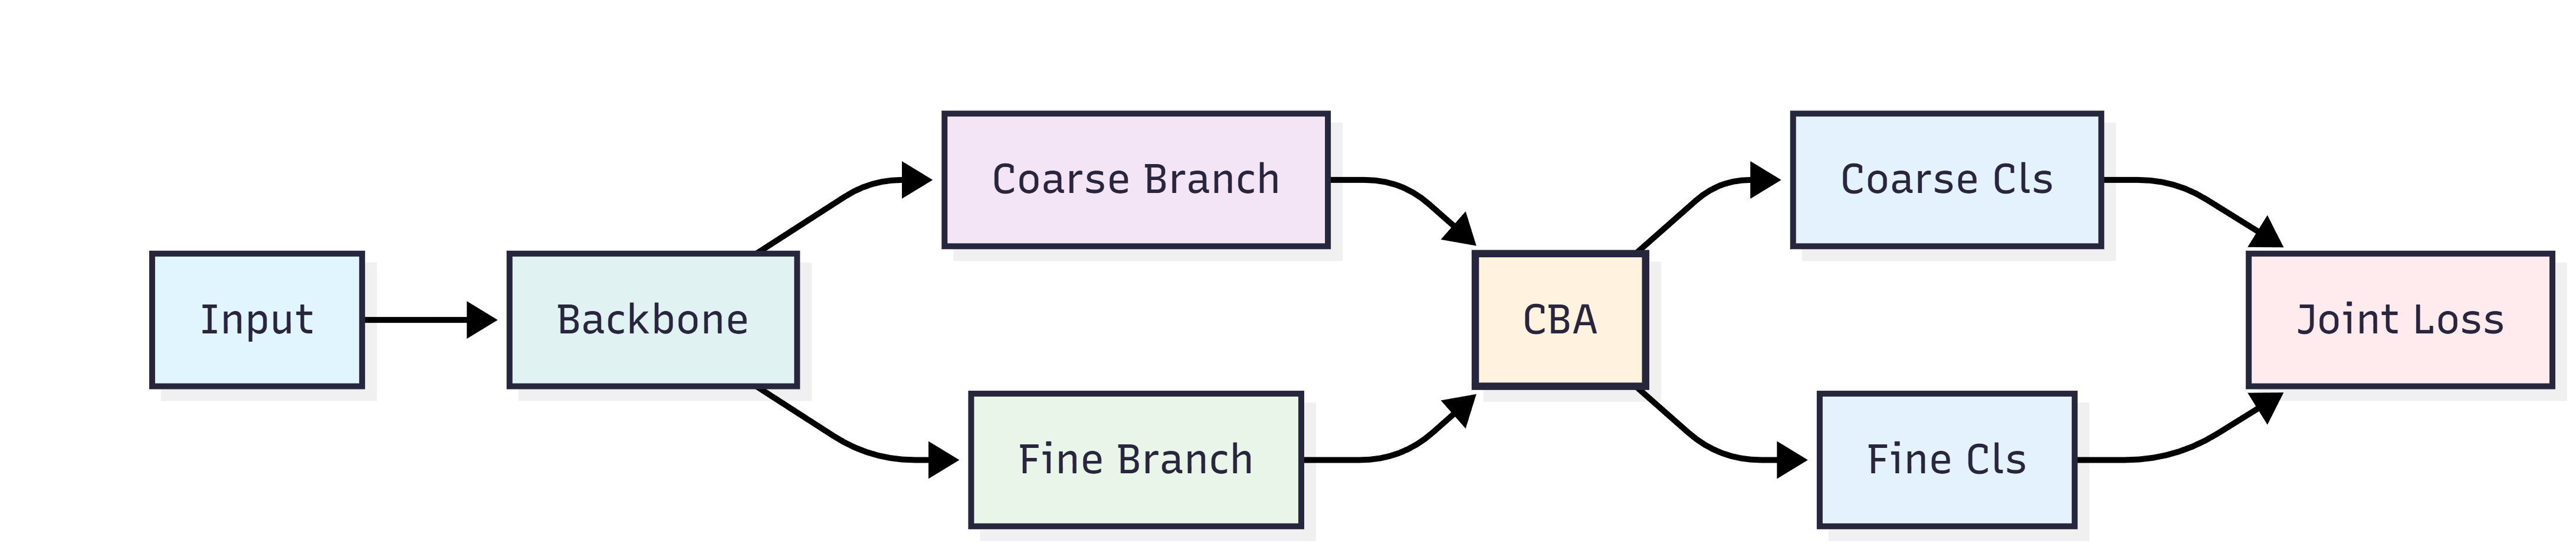
\includegraphics[width=\columnwidth]{imgs/model.png}
    \caption{Overview of HFENet, including the shared backbone, the coarse branch, the fine branch, and the associated training objectives.}
    \label{fig:architecture}
\end{figure}


\subsection{Cross-Branch Attention Mechanism}
\label{sec:cba}

\subsubsection{Design Motivation}

Conventional attention modules such as SE and CBAM mainly recalibrate features within the same branch. Although effective for enhancing local saliency, they do not explicitly model the directional dependency that coarse-grained semantics should constrain fine-grained discrimination in hierarchical recognition tasks. Simple feature concatenation or linear fusion is also insufficient, because it lacks adaptive conditioning and may introduce redundant information sharing across branches.

To address this issue, we design a cross-branch attention mechanism that uses coarse-level semantics as conditional guidance for fine-grained feature modulation. From an information conditioning perspective, this mechanism can be interpreted as increasing the discriminative utility of fine-grained representations under the guidance of coarse semantics:
\begin{equation}
I(\mathbf{F}_f'; y_f \mid \mathbf{F}_c),
\end{equation}
where $\mathbf{F}_f'$ denotes the modulated fine-grained features.

\subsubsection{Mechanism Implementation}
To enable conditional semantic guidance, we design a cross-branch attention module that uses coarse features to modulate fine features. 
The coarse feature $\mathbf{F}_c$ is compressed into a channel attention vector $\mathbf{a}_c \in \mathbb{R}^{1\times1\times C}$ and a spatial attention map $\mathbf{A}_s \in \mathbb{R}^{H \times W \times 1}$. 
By broadcast multiplication, they are combined into a channel-spatial modulation mask
\begin{equation}
\mathbf{M} = 1 + \alpha \cdot (\mathbf{A}_s \odot \mathbf{a}_c),
\label{eq:attention_mask}
\end{equation}
where $\mathbf{M}\in\mathbb{R}^{H\times W\times C}$ and $\alpha$ is a learnable scalar. 
The fine-grained feature is then modulated as
\begin{equation}
\mathbf{F}_f' = \mathbf{F}_f \odot \mathbf{M}.
\label{eq:feature_modulation}
\end{equation}

This process implements spatially- and channel-wise adaptive guidance from the coarse branch to the fine branch.

\subsubsection{Comparison with Existing Attention Mechanisms}
To highlight the distinctiveness of our cross-branch attention, Table~\ref{tab:attention_comparison} compares it with several representative attention mechanisms.
\begin{table*}[htbp]
    \centering
    \caption{Comparison of CBA with representative attention mechanisms.}
    \label{tab:attention_comparison}
    \setlength{\tabcolsep}{4pt}
    \renewcommand{\arraystretch}{1.1}
    \small
    \begin{tabular}{@{}lccccc@{}}
    \toprule
    \textbf{Method} & \textbf{Input} & \textbf{Target} & \textbf{Hier.} & \textbf{Dyn.} & \textbf{Cost} \\
    \midrule
    SE-Net      & Single     & Same  & No   & Static  & $O(c^2/r)$ \\
    CBAM        & Single     & Same  & No   & Static  & $O(c^2/r + hwc)$ \\
    Non-local   & Single     & Same  & No   & Dynamic & $O((hw)^2c)$ \\
    Cross-attn. & Two-branch & Other & Weak & Dynamic & $O(hwc^2)$ \\
    \midrule
    \textbf{CBA (Ours)} & \textbf{Cross-level} & \textbf{Fine} & \textbf{Strong} & \textbf{Dynamic} & $\mathbf{O(c^2/r + hwc)}$ \\
    \bottomrule
    \end{tabular}
\end{table*}
As summarized in Table~\ref{tab:attention_comparison}, existing attention mechanisms mainly operate within a single branch or do not explicitly encode coarse-to-fine hierarchical conditioning. In contrast, the proposed CBA is designed for cross-branch modulation, where coarse-level semantics provide adaptive channel-spatial guidance to fine-grained representations.

\subsection{Orthogonality Regularization}
\label{sec:orth}

A dual-branch architecture does not automatically guarantee complementary representation learning. 
When both branches are optimized on the same input and related supervision signals, they may converge to overlapping feature subspaces, which weakens the benefit of hierarchical decomposition. 
Therefore, redundancy suppression is not merely an optional regularization term, but a necessary constraint for preserving functional differentiation between the coarse and fine branches.

To reduce cross-branch redundancy, we first project the coarse and fine features into a shared embedding space. 
For a mini-batch of $N$ samples, let $\mathbf{F}_c \in \mathbb{R}^{N \times d_c}$ and $\mathbf{F}_f \in \mathbb{R}^{N \times d_f}$ denote the batch-wise coarse and fine features, respectively. 
We introduce two linear projections $\phi_c(\cdot)$ and $\phi_f(\cdot)$ to obtain
\begin{equation}
\hat{\mathbf{F}}_c = \phi_c(\mathbf{F}_c), \qquad
\hat{\mathbf{F}}_f = \phi_f(\mathbf{F}_f),
\end{equation}
where $\hat{\mathbf{F}}_c, \hat{\mathbf{F}}_f \in \mathbb{R}^{N \times d}$ are mapped to the same feature dimension $d$.

The cross-branch correlation matrix is then defined as
\begin{equation}
\mathbf{C}_{cf} = \frac{1}{N}\hat{\mathbf{F}}_c^\top \hat{\mathbf{F}}_f.
\end{equation}
The orthogonality regularization is formulated as
\begin{equation}
\mathcal{L}_{\text{orth}} = \|\mathbf{C}_{cf}\|_F^2.
\label{eq:orth_loss}
\end{equation}

Minimizing Eq.~\eqref{eq:orth_loss} suppresses correlated responses between the two branches and encourages them to encode complementary rather than redundant information. 
This constraint is particularly important in dual-branch architectures with shared low-level features, where branch collapse toward similar representations can otherwise occur.

\subsection{Hierarchical Joint Optimization}

Let $\mathbf{z}_f \in \mathbb{R}^{C_f}$ and $\mathbf{z}_c \in \mathbb{R}^{C_c}$ denote the logits of the fine and coarse classifiers, respectively. 
Their posterior probabilities are defined as
\begin{equation}
\mathbf{p}_f = \mathrm{softmax}(\mathbf{z}_f), \qquad
\mathbf{p}_c = \mathrm{softmax}(\mathbf{z}_c).
\end{equation}

Because each fine-grained class belongs to exactly one coarse-grained category, the fine prediction can be aggregated into the coarse label space. 
Let $\mathcal{G}(k)$ denote the set of fine classes belonging to coarse class $k$. 
The induced coarse distribution from the fine classifier is defined as
\begin{equation}
\tilde{p}_c(k) = \sum_{j \in \mathcal{G}(k)} p_f(j), \qquad k=1,\dots,C_c.
\label{eq:fine_to_coarse}
\end{equation}

Based on this mapping, the hierarchical KL consistency loss is formulated as
\begin{equation}
\mathcal{L}_{\mathrm{KL}} = \sum_{k=1}^{C_c} \tilde{p}_c(k)\log\frac{\tilde{p}_c(k)}{p_c(k)+\varepsilon},
\label{eq:kl_loss}
\end{equation}
where $\varepsilon$ is a small constant for numerical stability. 
This term encourages semantic consistency between the fine-grained prediction and the coarse-grained prediction, thereby improving cross-level coherence during training.

The overall loss function combines fine-grained classification loss $\mathcal{L}_f$, coarse-grained classification loss $\mathcal{L}_c$, hierarchical KL consistency loss $\mathcal{L}_{\mathrm{KL}}$, and orthogonality regularization:
\begin{equation}
\mathcal{L}_{\text{total}} = \mathcal{L}_f + \lambda_c \mathcal{L}_c + \lambda_{\mathrm{KL}} \mathcal{L}_{\mathrm{KL}} + \lambda_{\mathrm{orth}} \mathcal{L}_{\mathrm{orth}},
\label{eq:total_loss}
\end{equation}
where $\lambda_c$, $\lambda_{\mathrm{KL}}$, and $\lambda_{\mathrm{orth}}$ are balancing hyperparameters.

The model is trained end-to-end using the overall objective in Eq.~\eqref{eq:total_loss}.

\section{Experiments}
\label{sec:experiments}

\subsection{Datasets and Evaluation Metrics}
We evaluate on CIFAR-100 and Stanford Cars. CIFAR-100 contains 100 fine classes grouped into 20 coarse super-classes. Stanford Cars contains 196 fine classes (car models) with coarse labels based on brand (49 brands). We use 30\%, 50\%, 80\%, and 100\% training ratios to evaluate data efficiency. Top-1 accuracy (\%) is reported as mean $\pm$ std over three runs.

\subsection{Implementation Details}
All models are implemented in PyTorch and trained from scratch. Backbone: WideResNet-16-8 for HFENet and baselines. Optimizer: AdamW (lr=0.001, weight decay=5e-4) with cosine annealing for 300 epochs. Batch size: 64. Data augmentation: random cropping, horizontal flipping, AutoAugment, and random erasing (p=0.5). Loss weights: $\lambda_c=0.5$, $\lambda_{\mathrm{KL}}=0.2$, $\lambda_{\mathrm{orth}}=0.0005$ (determined via grid search).

\subsection{Comparison with State-of-the-Art}
All comparison models are trained under a unified from-scratch protocol to evaluate relative data efficiency under limited supervision. 
Under this setting, HFENet consistently outperforms the baseline WRN-16-8 and the compared representative backbones across different training ratios. 
The gains are particularly pronounced in low-data settings, suggesting that hierarchical feature alignment provides a useful inductive bias when supervision is insufficient. 
It should be emphasized that Transformer and modern CNN backbones are evaluated here without large-scale pre-training. 
Therefore, the results are mainly intended to compare data efficiency under a unified training regime, rather than to establish a universal ranking across different model families.

\begin{table*}[htbp]
    \centering
    \caption{Classification accuracy (\%) on CIFAR-100 under different training ratios.}
    \label{tab:cifar100_data_ratio}
    \begin{tabular}{@{}lcccc@{}}
    \toprule
    \textbf{Method} & \textbf{30\% data} & \textbf{50\% data} & \textbf{80\% data} & \textbf{100\% data} \\
    \midrule
    WRN-16-8 (Baseline) & 58.4 ± 0.3 & 68.7 ± 0.4 & 76.3 ± 0.2 & 80.2 ± 0.2 \\
    Dual-branch WRN (no interaction) & 61.6 ± 0.4 & 70.7 ± 0.3 & 78.2 ± 0.3 & 80.6 ± 0.2 \\
    ResNet50 & 55.2 ± 0.5 & 64.8 ± 0.4 & 72.5 ± 0.3 & 76.8 ± 0.3 \\
    DenseNet121 & 57.6 ± 0.4 & 66.9 ± 0.3 & 74.1 ± 0.3 & 78.3 ± 0.2 \\
    EfficientNet-B0 & 56.8 ± 0.5 & 66.2 ± 0.4 & 73.7 ± 0.3 & 77.9 ± 0.3 \\
    ViT-B & 39.5 ± 0.7 & 49.4 ± 0.6 & 64.6 ± 0.4 & 69.7 ± 0.4 \\
    Swin-T & 52.7 ± 0.6 & 59.7 ± 0.5 & 66.2 ± 0.4 & 69.1 ± 0.3 \\
    PVTv2 & 48.3 ± 0.6 & 56.9 ± 0.5 & 63.8 ± 0.4 & 67.5 ± 0.4 \\
    ConvNeXt-V2 & 53.8 ± 0.5 & 62.4 ± 0.4 & 69.1 ± 0.3 & 72.6 ± 0.3 \\
    \hline
    \textbf{HFENet (Ours)} & \textbf{70.8 ± 0.3} & \textbf{77.2 ± 0.2} & \textbf{80.5 ± 0.2} & \textbf{82.7 ± 0.2} \\
    \bottomrule
    \end{tabular}
\end{table*}

Results in Table~\ref{tab:cifar100_data_ratio} show that HFENet consistently improves over the baseline WRN-16-8 and the dual-branch variant without interaction across all training ratios. 
The improvement is particularly significant in low-data settings, where HFENet exceeds WRN-16-8 by 12.4 points at 30\% data and 8.5 points at 50\% data. 
The margin becomes smaller at 100\% data, which suggests that the benefit of hierarchical alignment is most pronounced when the amount of supervision is limited. 
Notably, HFENet at 50\% data already surpasses the full-data performance of WRN-16-8, further indicating its advantage in data-efficient learning.

\subsubsection{Convergence Analysis}
Convergence curves in Fig.~\ref{fig:convergence_curves} further illustrate the optimization behavior. HFENet achieves faster initial convergence and better final accuracy, demonstrating the benefit of hierarchical guidance and redundancy suppression.
\begin{figure*}[htbp]
    \centering
    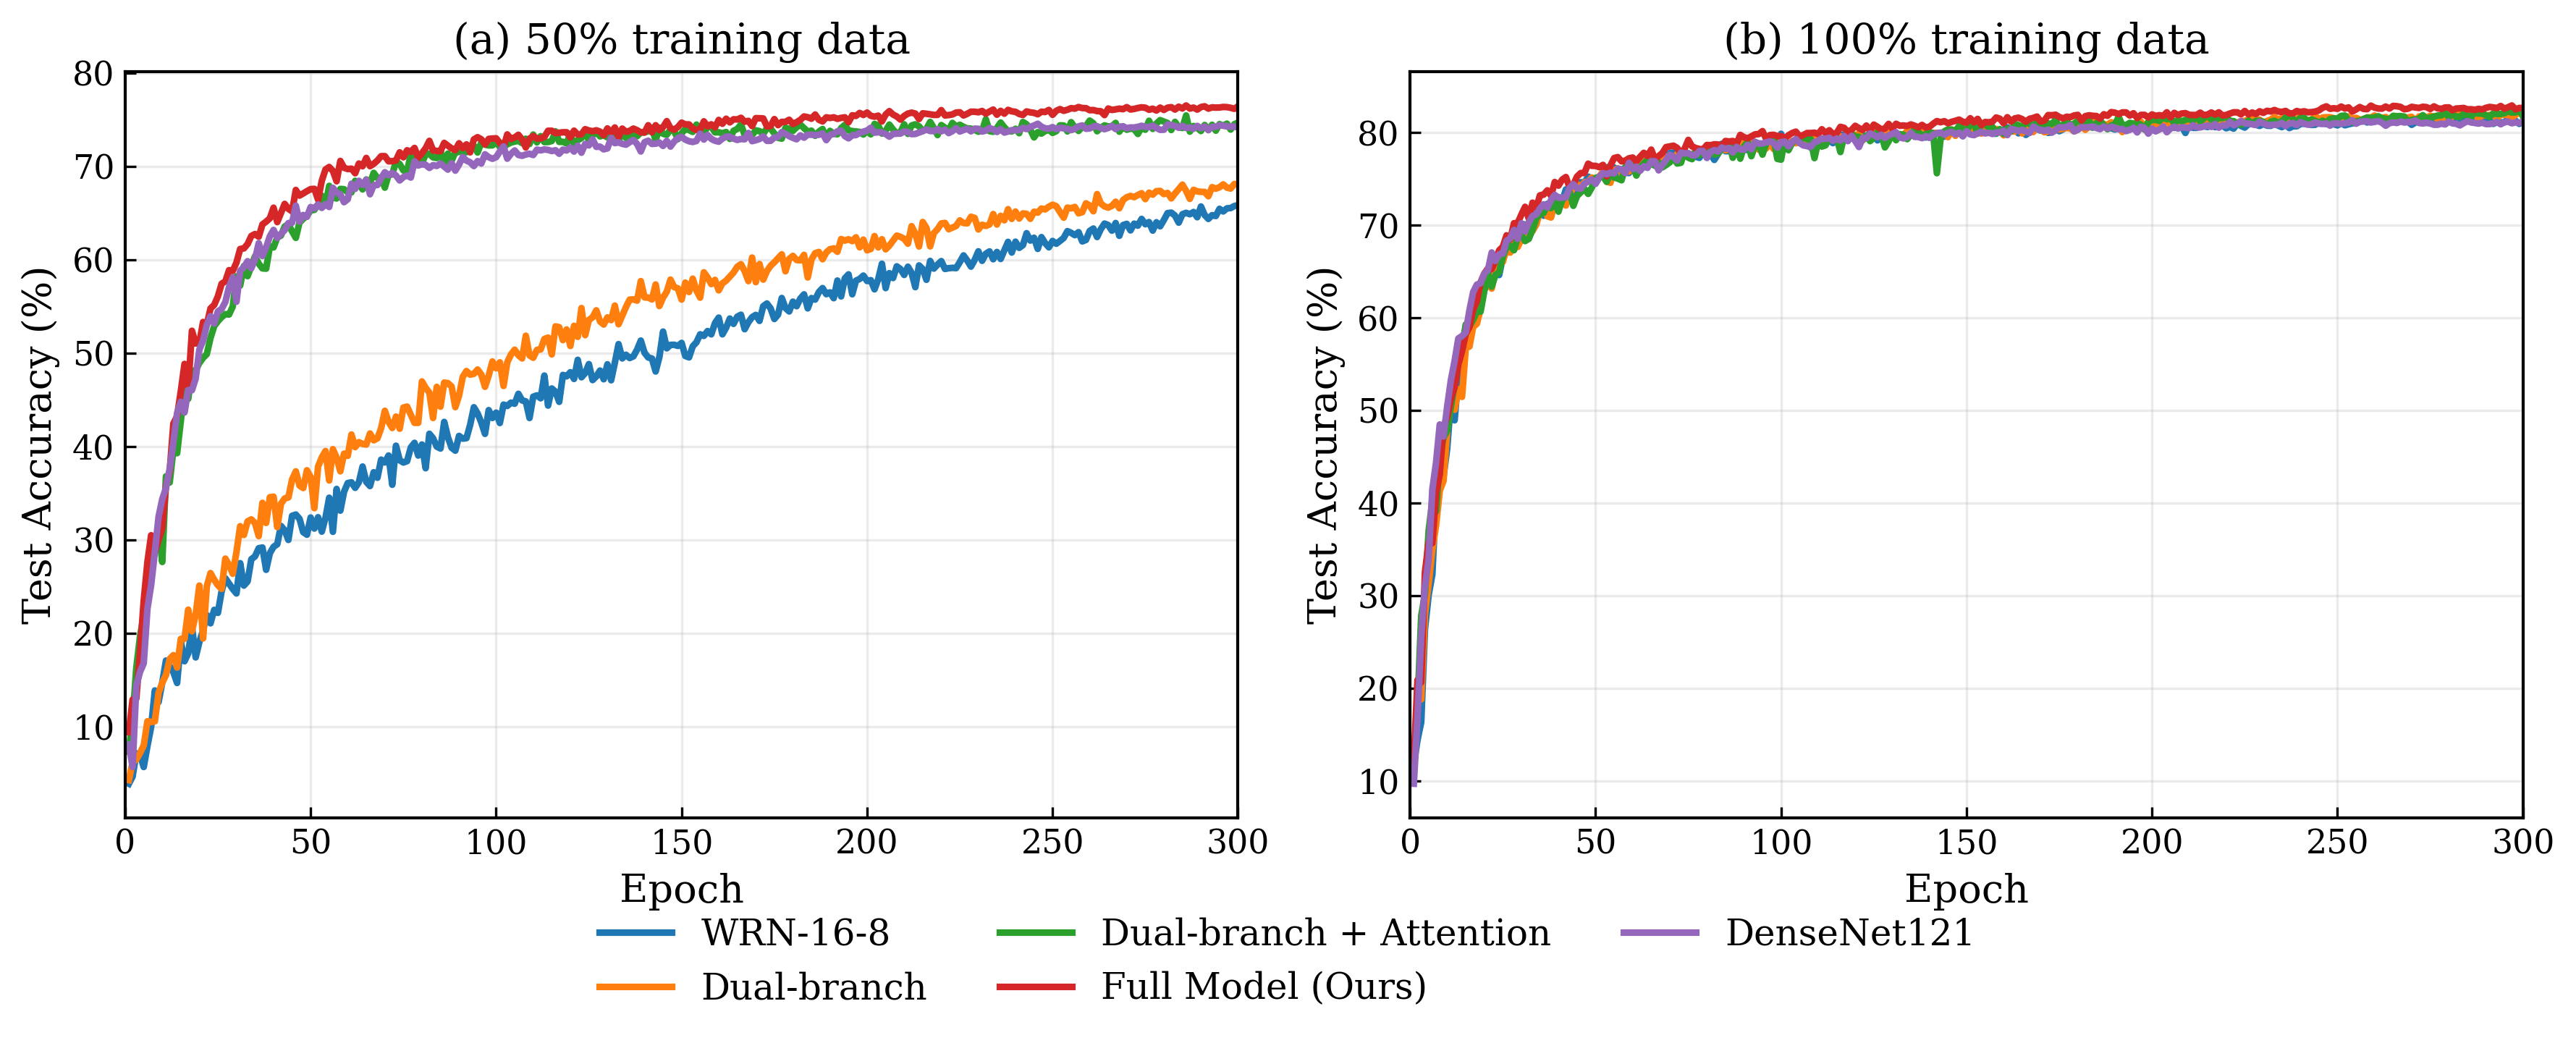
\includegraphics[width=\textwidth]{imgs/convergence_curves_final_paper.png}
    \caption{Test accuracy convergence curves on CIFAR-100 with 50\% and 100\% training data.}
    \label{fig:convergence_curves}
\end{figure*}

\subsection{Results on Stanford Cars}
To provide preliminary evidence of generalizability, we further evaluate HFENet on Stanford Cars, an additional fine-grained benchmark with 196 model classes and 49 brand-level coarse categories. Results are shown in Table~\ref{tab:cars_results}.
\begin{table*}[htbp]
    \centering
    \caption{Classification accuracy (\%) on Stanford Cars.}
    \label{tab:cars_results}
    \begin{tabular}{@{}lcc@{}}
    \toprule
    \textbf{Method} & \textbf{50\% data} & \textbf{100\% data} \\
    \midrule
    WRN-16-8 (Baseline) & 50.52 ± 0.6 & 81.17 ± 0.3 \\
    Dual-branch WRN (no interaction) & 62.48 ± 0.5 & 82.24 ± 0.3 \\
    Dual-branch + CBA & 63.25 ± 0.4 & 83.04 ± 0.2 \\
    \textbf{HFENet (Ours)} & \textbf{65.73 ± 0.4} & \textbf{83.95 ± 0.2} \\
    \hline
    ResNet50 & 42.07 ± 0.7 & 80.06 ± 0.4 \\
    DenseNet121 & 49.12 ± 0.6 & 82.31 ± 0.3 \\
    \bottomrule
    \end{tabular}
\end{table*}
HFENet achieves the best performance among the compared methods on Stanford Cars in both training settings. 
Compared with WRN-16-8, the proposed method improves accuracy by 15.21 points at 50\% data and by 2.78 points at 100\% data, indicating that hierarchical feature alignment remains beneficial beyond CIFAR-100. 
Since the comparison set on Stanford Cars is smaller than that on CIFAR-100, these results should be regarded as supplementary evidence of generalizability rather than an exhaustive benchmark study.

\subsection{Ablation Studies}
We conduct ablations on CIFAR-100 to isolate the contribution of each component. Results are presented in Table~\ref{tab:ablation_all}.

\begin{table*}[htbp]
    \centering
    \caption{Ablation results on CIFAR-100 under different training ratios (\% accuracy).}
    \label{tab:ablation_all}
    \setlength{\tabcolsep}{4pt}
    \renewcommand{\arraystretch}{1.1}
    \small
    \begin{tabular}{@{}lccccc@{}}
    \toprule
    \textbf{Ratio} & \textbf{WRN-16-8} & \textbf{Dual} & \textbf{Dual+CBA} & \textbf{Dual+Orth.} & \textbf{Full} \\
    \midrule
    30\%  & 58.4 $\pm$ 0.3 & 61.6 $\pm$ 0.4 & 69.9 $\pm$ 0.3 & 62.3 $\pm$ 0.2 & \textbf{70.8 $\pm$ 0.3} \\
    50\%  & 68.7 $\pm$ 0.4 & 70.7 $\pm$ 0.3 & 75.3 $\pm$ 0.3 & 71.2 $\pm$ 0.3 & \textbf{77.2 $\pm$ 0.2} \\
    80\%  & 76.3 $\pm$ 0.2 & 78.2 $\pm$ 0.3 & 79.2 $\pm$ 0.2 & 78.8 $\pm$ 0.2 & \textbf{80.5 $\pm$ 0.2} \\
    100\% & 80.2 $\pm$ 0.2 & 80.6 $\pm$ 0.2 & 82.1 $\pm$ 0.2 & 81.2 $\pm$ 0.2 & \textbf{82.7 $\pm$ 0.2} \\
    \bottomrule
    \end{tabular}
\end{table*}

Dual-branch decomposition alone yields limited improvements over the baseline, indicating that merely separating coarse- and fine-level pathways is insufficient. 
Introducing CBA brings substantial gains, which confirms the importance of explicit coarse-to-fine semantic guidance. 
Adding orthogonality regularization further improves performance by suppressing redundant cross-branch representations. 
The full model achieves the best results across all training ratios, suggesting that hierarchical alignment and redundancy suppression are complementary rather than interchangeable.

\subsection{Feature Correlation Analysis}

To examine whether orthogonality regularization effectively reduces branch-wise redundancy, we visualize the correlation patterns of dual-branch features with and without the proposed regularization. 
As shown in Fig.~\ref{fig:correlation_analysis}, the model without orthogonality regularization exhibits stronger cross-branch correlation, indicating that the two branches tend to encode overlapping information. 
After introducing orthogonality regularization, the overall correlation magnitude is reduced, which suggests that the coarse and fine branches become more complementary.

\begin{figure}[!t]
    \centering
    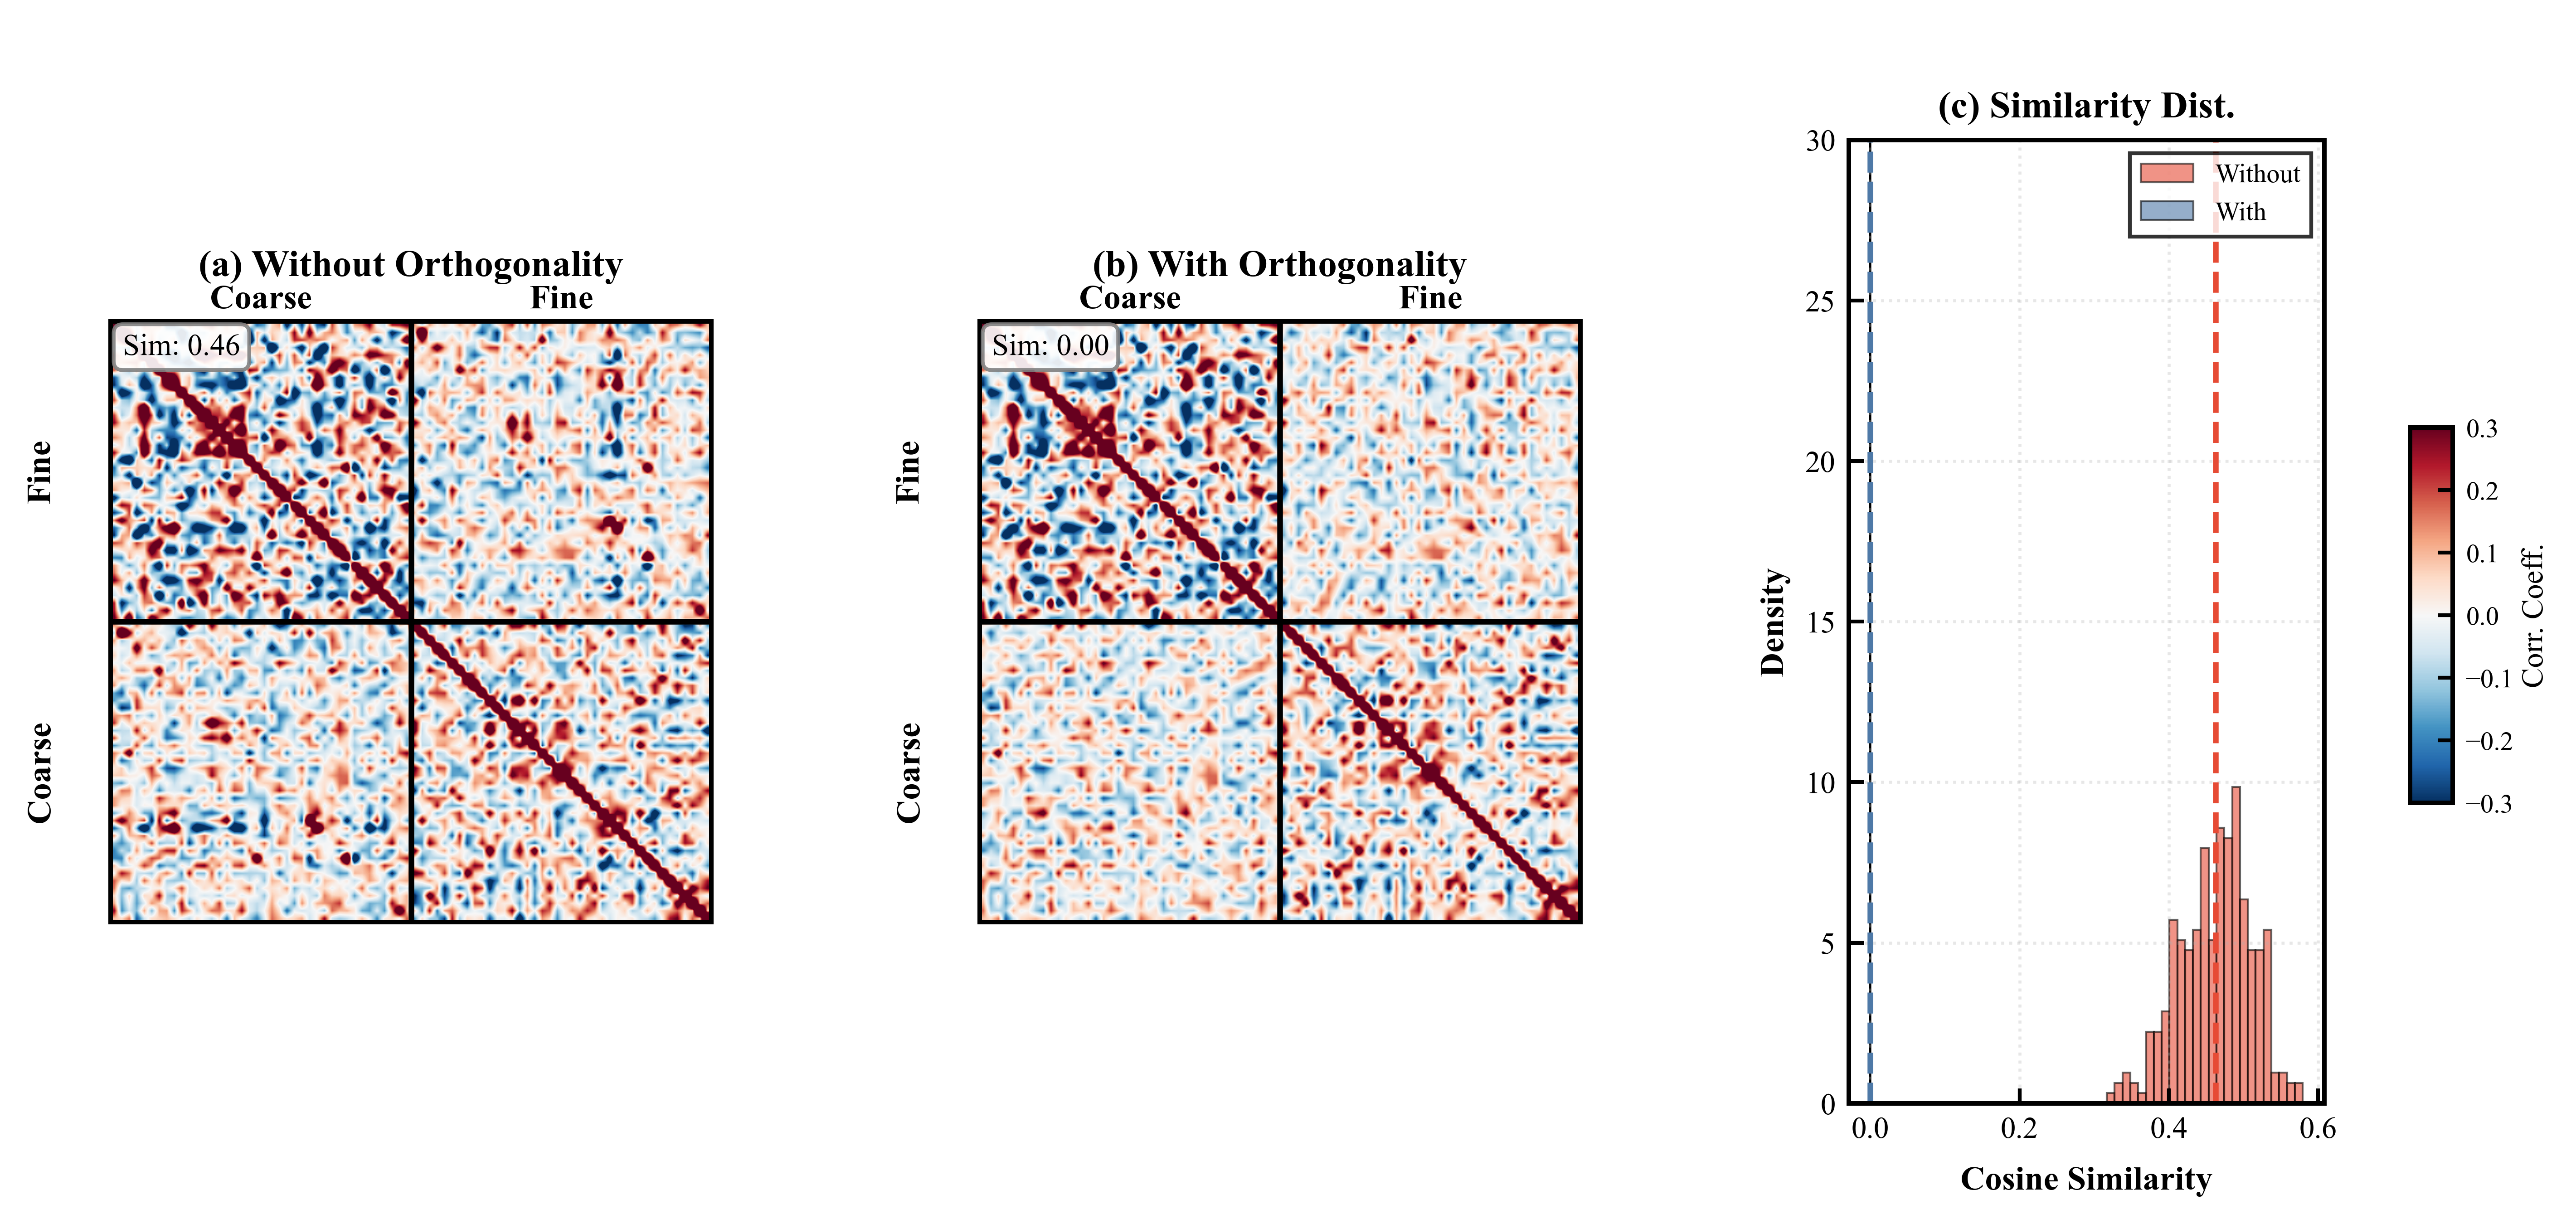
\includegraphics[width=0.9\columnwidth]{imgs/fig2_combined.png}
    \caption{Feature correlation analysis of dual-branch representations with and without orthogonality regularization. The regularized model exhibits weaker cross-branch correlation, indicating reduced redundancy and stronger complementarity.}
    \label{fig:correlation_analysis}
\end{figure}

This observation is consistent with the ablation results in Table~\ref{tab:ablation_all}, where adding orthogonality regularization yields further gains over the plain dual-branch architecture. 
These results support the claim that redundancy suppression is beneficial for preserving functional differentiation between the two branches.

\FloatBarrier

\subsection{Visualization Analysis}

We visualize Grad-CAM heatmaps on CIFAR-100 (Fig.~\ref{fig:grad_cam_vis}) and Stanford Cars (Fig.~\ref{fig:cars_gradcam}) to qualitatively examine the effect of hierarchical feature alignment. 
Compared with WRN-16-8, HFENet tends to produce more target-focused responses and is less easily distracted by background regions or irrelevant structures.

\begin{figure*}[!t]
    \centering
    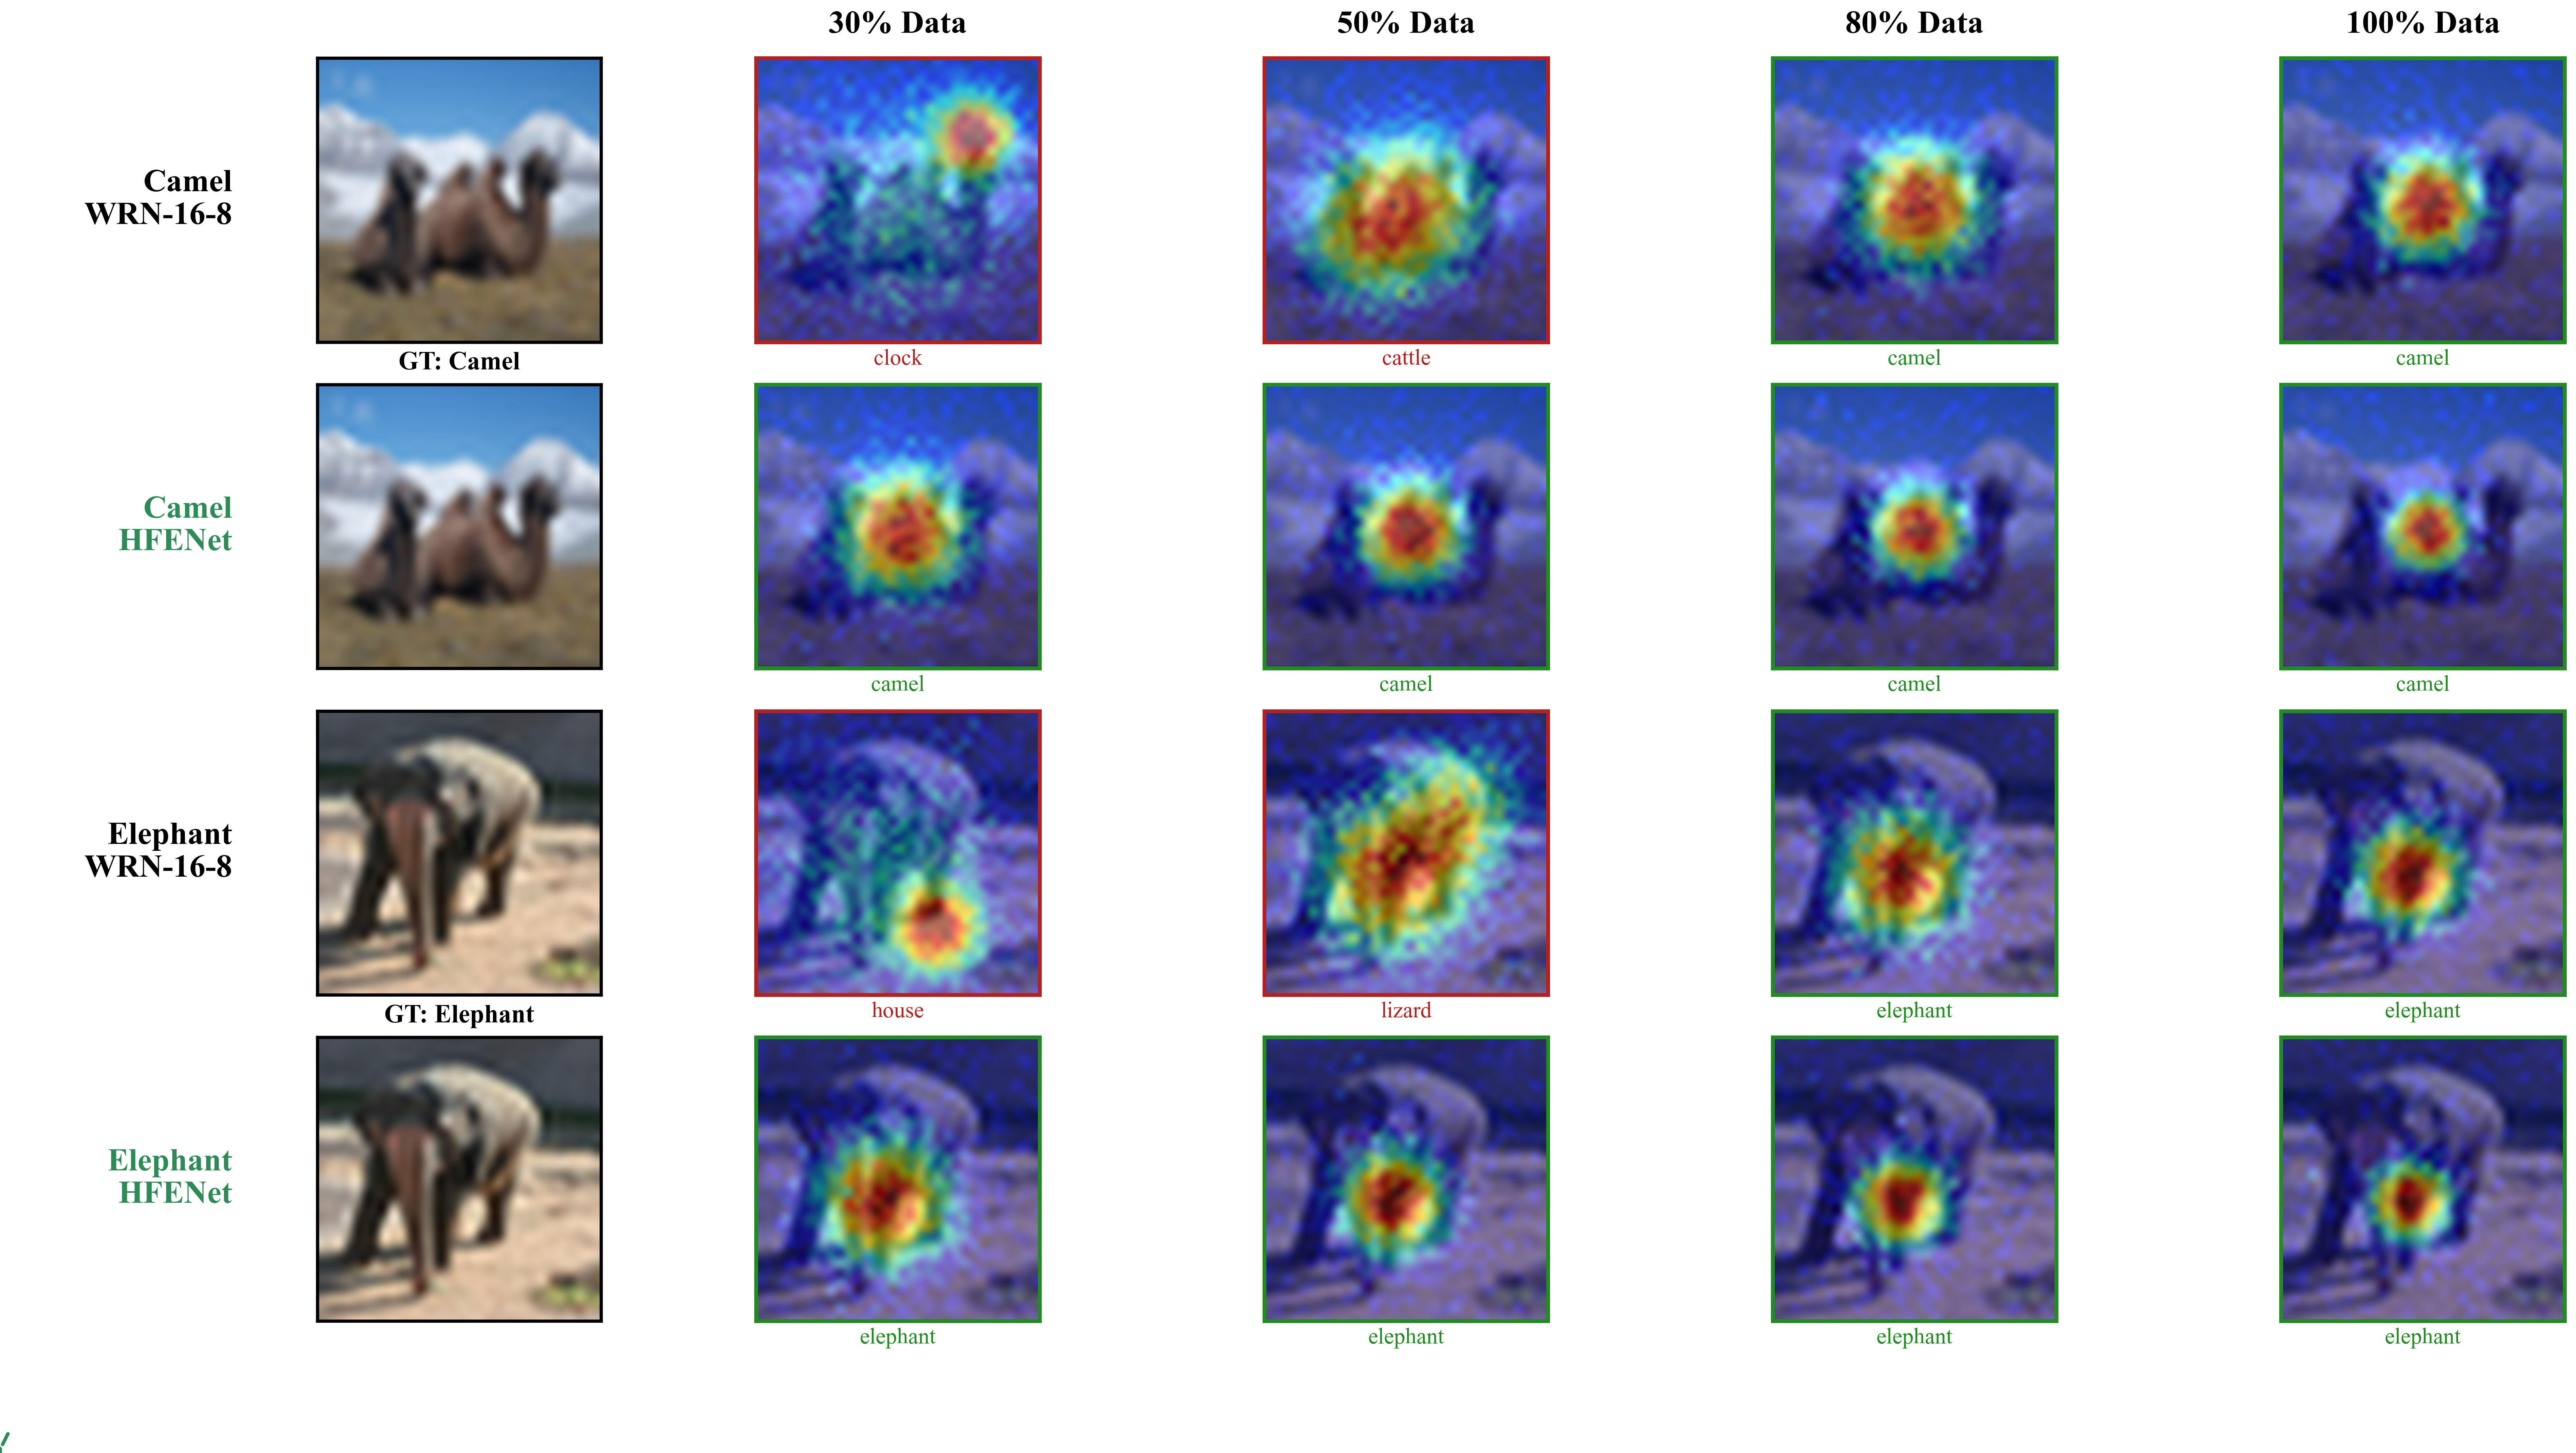
\includegraphics[width=\textwidth]{imgs/fig3_sci_q4_comparison_two_classes.png}
    \caption{Grad-CAM comparison between WRN-16-8 and HFENet on CIFAR-100 under different training ratios.}
    \label{fig:grad_cam_vis}
\end{figure*}

On CIFAR-100, the attention maps of HFENet are generally more concentrated on the object body and its discriminative parts, whereas the baseline model often produces scattered or background-sensitive responses. 
This difference is more evident under reduced training ratios, which is consistent with the quantitative results showing stronger gains in limited-data settings. 
These visualizations suggest that coarse-to-fine semantic guidance helps stabilize discriminative localization when fine-grained supervision is insufficient.

\begin{figure}[!t]
    \centering
    \includegraphics[width=\columnwidth]{imgs/fig3_stanford_cars_two_classes.png}
    \caption{Grad-CAM comparison between WRN-16-8 and HFENet on Stanford Cars.}
    \label{fig:cars_gradcam}
\end{figure}

A similar trend can also be observed on Stanford Cars, where HFENet focuses more consistently on category-relevant regions such as the vehicle body and local structural cues. 
This qualitative evidence further supports the role of hierarchical alignment in improving fine-grained representation learning.

\subsection{Error Analysis}

We further inspect representative failure cases of HFENet on CIFAR-100 to better understand its remaining limitations. 
Most misclassifications can be grouped into three categories. 
First, severe occlusion of discriminative parts prevents the fine branch from capturing reliable local evidence. 
Second, some categories exhibit extremely subtle inter-class differences, for which coarse-level guidance alone is insufficient to resolve ambiguity. 
Third, low-resolution samples limit the availability of local structural details and reduce the effectiveness of fine-grained discrimination.

These observations indicate that, although hierarchical guidance improves branch coordination and discriminative focus, the model still depends on sufficiently visible local cues. 
They also suggest that future improvement may require stronger part-aware modeling, higher-resolution feature extraction, or more robust local detail enhancement.

\section{Discussion}
\label{sec:discussion}

\subsection{Advantages of the Proposed Method}
HFENet improves data efficiency by jointly addressing two issues in hierarchical fine-grained learning: insufficient semantic coordination across levels and feature redundancy across branches. The proposed cross-branch attention allows coarse-level semantics to condition fine-grained feature modulation, which helps stabilize discriminative learning when training data are limited. Meanwhile, orthogonality regularization reduces redundant responses between the two branches and encourages a more complementary division of representation roles. Taken together, these two components provide a structured way to couple semantic guidance with redundancy suppression in dual-branch fine-grained classification.

\subsection{Practical Application Scenarios}
HFENet is particularly suitable for scenarios with natural or definable category hierarchies and limited training samples. Potential applications include:
\begin{itemize}
    \item Industrial defect inspection, where product categories are naturally hierarchical (e.g., type of defect, severity level) and labeled data is often scarce.
    \item Species recognition in biology, where coarse taxonomic ranks (genus, family) can guide fine-grained species identification.
    \item Fine-grained product recognition in e-commerce, where brand-level semantics help differentiate similar models.
\end{itemize}
It is worth noting that this work does not systematically evaluate efficiency in resource-constrained deployment (e.g., edge devices), and its practical applicability in such settings remains for future investigation.

\subsection{Limitations and Future Work}
Current limitations include:
\begin{itemize}
    \item Reliance on predefined hierarchical labels; the method may not directly apply when such labels are absent.
    \item Introduction of additional hyperparameters ($\lambda_c$, $\lambda_{\mathrm{KL}}$, $\lambda_{\mathrm{orth}}$), which require tuning on a validation set.
    \item Evaluation is limited to CIFAR-100 and Stanford Cars; broader fine-grained datasets (e.g., iNaturalist, NABirds) should be tested.
\end{itemize}
Future work will focus on: (1) extending the framework to more diverse fine-grained benchmarks; (2) exploring adaptive or self-supervised hierarchy discovery; (3) designing more efficient implementations of attention and orthogonality constraints; (4) transferring the hierarchical alignment idea to other vision tasks such as object detection and segmentation; and (5) investigating semi-supervised or weakly-supervised settings where hierarchy labels are only partially available.

\section{Conclusion}
\label{sec:conclusion}
This paper proposed HFENet, a dual-branch framework for fine-grained image classification built around the central idea of hierarchical feature alignment for coarse-to-fine representation learning. 
Within this framework, cross-branch attention enables directional semantic guidance from the coarse branch to the fine branch, while orthogonality regularization suppresses redundant cross-branch representations and promotes complementarity. 
Hierarchical KL consistency further improves semantic coherence during training. 
Experimental results on CIFAR-100 and Stanford Cars show that HFENet consistently improves recognition performance, especially under limited-data settings. 
These findings suggest that explicitly combining hierarchical alignment and redundancy suppression is a promising direction for data-efficient fine-grained recognition.

\section*{Acknowledgements}
We thank our laboratory colleagues for valuable discussions and the anonymous reviewers for their constructive comments. This work was supported by the XXX Foundation (Grant No. XXXX).

\begin{thebibliography}{50}

\bibitem{du2020fine} Du, R., Chang, D., Bhunia, A. K., Xie, J., Ma, Z., Song, Y. Z., \& Guo, J. (2020). Fine-grained visual classification via progressive multi-granularity training. In \textit{European Conference on Computer Vision} (pp. 137-153). Springer, Cham.

\bibitem{yan2015hdcnn} Yan, Z., Zhang, H., Piramuthu, R., Jagadeesh, V., DeCoste, D., Di, W., \& Yu, Y. (2015). HD-CNN: hierarchical deep convolutional neural network for large scale visual recognition. In \textit{Proceedings of the IEEE International Conference on Computer Vision} (pp. 2740-2748).

\bibitem{hu2018squeeze} Hu, J., Shen, L., \& Sun, G. (2018). Squeeze-and-excitation networks. In \textit{Proceedings of the IEEE Conference on Computer Vision and Pattern Recognition} (pp. 7138-7141).

\bibitem{woo2018cbam} Woo, S., Park, J., Lee, J. Y., \& Kweon, I. S. (2018). CBAM: Convolutional block attention module. In \textit{Proceedings of the European Conference on Computer Vision} (pp. 3-19).

\bibitem{zheng2017learning} Zheng, H., Fu, J., Mei, T., \& Luo, J. (2017). Learning multi-attention convolutional neural network for fine-grained image recognition. In \textit{Proceedings of the IEEE International Conference on Computer Vision} (pp. 5209-5217).

\bibitem{fu2017look} Fu, J., Zheng, H., \& Mei, T. (2017). Look closer to see better: Recurrent attention convolutional neural network for fine-grained image recognition. In \textit{Proceedings of the IEEE Conference on Computer Vision and Pattern Recognition} (pp. 4438-4446).

\bibitem{he2021transfg} He, J., Chen, J. N., Liu, S., Kortylewski, A., Yang, C., Bai, Y., \& Wang, C. (2021). Transfg: A transformer architecture for fine-grained recognition. In \textit{Proceedings of the AAAI Conference on Artificial Intelligence} (Vol. 36, No. 1, pp. 852-860).

\bibitem{part_rcnn} Zhang, N., Donahue, J., Girshick, R., \& Darrell, T. (2014). Part-based R-CNNs for fine-grained category detection. In \textit{European Conference on Computer Vision} (pp. 834-849). Springer, Cham.

\bibitem{bilinear_cnn} Lin, T. Y., RoyChowdhury, A., \& Maji, S. (2015). Bilinear CNN models for fine-grained visual recognition. In \textit{Proceedings of the IEEE International Conference on Computer Vision} (pp. 1449-1457).

\bibitem{nonlocal} Wang, X., Girshick, R., Gupta, A., \& He, K. (2018). Non-local neural networks. In \textit{Proceedings of the IEEE Conference on Computer Vision and Pattern Recognition} (pp. 7794-7803).

\bibitem{dosovitskiy2020image} Dosovitskiy, A., Beyer, L., Kolesnikov, A., Weissenborn, D., Zhai, X., Unterthiner, T., ... \& Houlsby, N. (2020). An image is worth 16x16 words: Transformers for image recognition at scale. \textit{arXiv preprint arXiv:2010.11929}.

\bibitem{liu2021swin} Liu, Z., Lin, Y., Cao, Y., Hu, H., Wei, Y., Zhang, Z., ... \& Guo, B. (2021). Swin transformer: Hierarchical vision transformer using shifted windows. In \textit{Proceedings of the IEEE/CVF International Conference on Computer Vision} (pp. 10012-10022).

\bibitem{touvron2021training} Touvron, H., Cord, M., Douze, M., Massa, F., Sablayrolles, A., \& Jégou, H. (2021). Training data-efficient image transformers \& distillation through attention. In \textit{International Conference on Machine Learning} (pp. 10347-10357). PMLR.

\bibitem{liu2022convnext} Liu, Z., Mao, H., Wu, C. Y., Feichtenhofer, C., Darrell, T., \& Xie, S. (2022). A convnet for the 2020s. In \textit{Proceedings of the IEEE/CVF Conference on Computer Vision and Pattern Recognition} (pp. 11976-11986).

\bibitem{wang2022pvt} Wang, W., Xie, E., Li, X., Fan, D. P., Song, K., Liang, D., ... \& Shao, L. (2022). PVT v2: Improved baselines with pyramid vision transformer. \textit{Computational Visual Media}, 8(3), 415-424.

\bibitem{woo2023convnextv2} Woo, S., Debnath, S., Hu, R., Chen, X., Liu, Z., Kweon, I. S., \& Xie, S. (2023). ConvNeXt V2: Co-designing and scaling ConvNets with masked autoencoders. In \textit{Proceedings of the IEEE/CVF Conference on Computer Vision and Pattern Recognition} (pp. 16133--16142).

\bibitem{wang2025crasmra} Wang, X., Sun, Y., Liu, X., Zou, Z., Wang, L., Wang, K., Liang, X., \& Liu, W. (2025). Rethinking attention mechanism: Channel re-attention and spatial multi-region attention for fine-grained visual classification. \textit{Neural Processing Letters}, 57, 43.

\bibitem{wang2025cfgvc} Wang, Y., Wang, Y., Ye, Q., Lang, W., \& Xu, C. (2025). Strengthen contrastive semantic consistency for fine-grained image classification. \textit{Pattern Analysis and Applications}, 28, 75.

\bibitem{gao2025chbc} Gao, P., Liang, Y., Song, Y., \& Yang, Z. (2025). Cross-hierarchical bidirectional consistency learning for fine-grained visual classification. \textit{Information Sciences}, 721, 122562.

\bibitem{xie2025dotcbm} Xie, Y., Zeng, Z., Zhang, H., Ding, Y., Wang, Y., Wang, Z., Chen, B., \& Liu, H. (2025). Discovering fine-grained visual-concept relations by disentangled optimal transport concept bottleneck models. In \textit{Proceedings of the IEEE/CVF Conference on Computer Vision and Pattern Recognition}.

\bibitem{park2025freegrained} Park, S., Wang, Z., \& Yu, S. X. (2025). Free-grained hierarchical recognition. \textit{arXiv preprint arXiv:2510.14737}.

\bibitem{sikdar2025interweaving} Sikdar, A., Liu, Y., Kedarisetty, S., et al. (2025). Interweaving insights: high-order feature interaction for fine-grained visual recognition. \textit{International Journal of Computer Vision}, 133, 1755--1779.
\end{thebibliography}

\end{document}